\subsection{Problems}
\begin{tcolorbox}
\noindent {\bf Problem \thesection.\theprob}\stepcounter{prob}

The outer diameter of a CPU axial cooler ventilator is $D_o=47\,\mathrm{mm}$ the inner diameter is $D_i=21.5\,\mathrm{mm}$ the revolution speed is $n=2740\,\mathrm{rpm}$. Due to the careful design the hydraulic efficiency is $\eta_h=85\%$ however the volumetric efficiency as consequence of leakage flow rate between the housing and the impeller is just $\eta_{vol}=75\%$. The blade angle at the suction side is $\beta_1=20^\circ$ while at the pressure side $\beta_2=40^\circ$. Find the flow rate and the total pressure rise on the impeller. The density of the air is $\rho=1.25\,\mathrm{kg/m^3}$. Draw the velocity triangles at the inlet and the outlet at the mean diameter.
%
\begin{itemize}
\item $A_{ring}=\frac{\left(D_o^2-D_i^2\right)\pi}{4}=0.00137\,\mathrm{m^2}$
\item $D_{mean}=\frac{D_o+D_i}{2}=0.03425\,\mathrm{m}$
\item $u_{mean}=u_1=u_2=D_{mean}\pi n=4.913\,\mathrm{\frac{m}{s}}$
\item $c_{ax}=c_{1,ax}=c_{2,ax}=u \tan\beta_1=1.788\,\mathrm{\frac{m}{s}}$
\item $q=\eta_{vol}A_{ring}c_{ax}=0.00184\,\mathrm{\frac{m^3}{s}}$
\item $w_{2u}=\frac{c_{ax}}{\tan\beta_2}=2.131\,\mathrm{\frac{m}{s}}$
\item $\Delta c_u=u-w_{2u}=2.782\,\mathrm{\frac{m}{s}}$
\item $\Delta p_{total,ideal}=\rho u\Delta c_u=17.1\,\mathrm{Pa}$
\item $\Delta p_{total}=\eta_h \Delta p_{total,ideal}=14.5\,\mathrm{Pa}$
\end{itemize}
\end{tcolorbox}
	
\vspace{1cm}
\begin{tcolorbox}
\noindent {\bf Problem \thesection.\theprob}\stepcounter{prob}

The inner diameter of an axial impeller is $D_i=250$ mm, while the outer one is $D_o=400$mm. The revolution number of the impeller is $1470$rpm. The inlet is prerotation-free. At $Q=0.36\,\mathrm{ m^3/s}$ the hydraulic efficiency is 85\%, the head is 6 m. The specific work along the radius is constant. Find the angles $\beta_{1,2}$  at the inner and outer diameter. 


%(Solution: $\beta_{1,i}=13.7$, $\beta_{2,i}=16.7$, $\beta_{1,o}=8.7$ and $\beta_{2,o}=9.4$ degrees) 
\vspace{0.2cm}

Solution:

\begin{itemize}
%
\item The velocity triangles are depicted in the Figure \ref{gen_vtr}.
%
\item The circumferential speed at the inner diameter is $u_{2i}=D_i\pi n=0.25\pi \frac{1470}{60}= 19.24 m/s$. The two circumferential speeds $u_{i,1}$ and $u_{i,2}$ equal as they are located at the same (inner) radius.
%
\item The circumferential speed at the outer diameter is $u_{20}=D_o\pi n=0.4\pi\frac{1470}{60}= 30.79 m/s$. Again the the two circumferential speeds $u_{o,1}$ and $u_{o,2}$ equal as they are located at the same (outer) radius.
%
\item The theoretical head is $H_{th}=\frac{c_{2u}u_2}{g}=\frac{H}{\eta_h}=7.059m$. We also have  $c_{2u}u_2=H_{th}g=69.247$ $m^2/s^2$, which is constant along the radius: $c_{2u,i}=\frac{69.247}{19.24}=3.56$ m/s and $c_{2u,o}=\frac{69.247}{30.79}=2.25$ m/s.
%
\item The axial component of the velocity is $c_{ax}=\frac{4Q}{\left({D_o}^2-{D_i}^2\right)\pi}=\frac{4 \times 0.36}{\left({0.4}^2-{0.25}^2\right)\pi}=4.70$ m/s
%
\item The blade angles are
\begin{equation*}
\beta_{1i}=\arctan\frac{c_{ax}}{u_{2i}}=
%=\arctan\frac{4.70}{19.24}=
13.73^o \quad \text{and}\quad \beta_{2i}=\arctan\frac{c_{ax}}{u_{2a}-c_{2ui}}
%=arctan\frac{4.70}{19.24-3.56}=
=16.7^o.
\end{equation*}

\item With the same train of thought, one obtains $\beta_{10}=8.7^o$ and $\beta_{20}=9.4^o$.
\end{itemize}
\end{tcolorbox}
\vspace{1cm}

\begin{figure}[ht]
\begin{center}
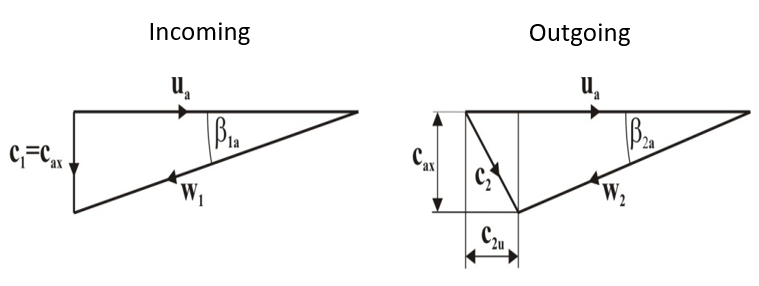
\includegraphics[scale=0.6]{figs/problem_2p2p16_vel_tri_fig.png}
\caption{\label{gen_vtr}Velocity triangles}
\end{center}
\end{figure}

